% translation-source: docs/user/latex/chapters/01-demarrage.tex; sha256: ef75f3d3a176fe7470c6c9d457e2df8fe9be18791e8a567cf18dab62e7f221d6
\chapter{First launch and orientation}
\label{chap:demarrage}
\section{Open a photo}
From the welcome screen, click \emph{Open…} and select an image.
IPR opens its containing folder and displays the folder's images in the bottom
filmstrip. The \emph{File / Open image…} and \emph{Open folder…} menus let you
switch photos or folders. Use \touche{Ctrl + O} for an image and
\touche{Ctrl + Shift + O} for a folder.

A RAW contains data that must be developed; a JPEG, PNG or TIFF already contains
a rendered image. A DNG can contain different kinds of data: its extension alone
does not establish that it contains a RAW mosaic. Use the dialog filters to see
which files the installed build offers.

\section{The four working areas}
\begin{center}
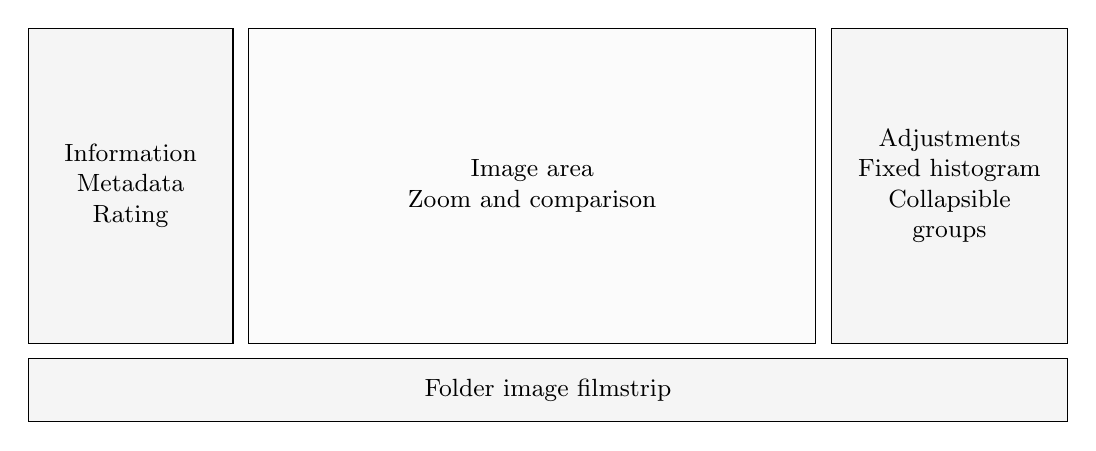
\begin{tikzpicture}[x=1cm,y=1cm,every node/.style={font=\small,align=center}]
\draw[fill=gray!8] (0,1) rectangle (2.6,5);
\draw[fill=gray!3] (2.8,1) rectangle (10,5);
\draw[fill=gray!8] (10.2,1) rectangle (13.2,5);
\draw[fill=gray!8] (0,0) rectangle (13.2,0.8);
\node at (1.3,3) {Information\\Metadata\\Rating};
\node at (6.4,3) {Image area\\Zoom and comparison};
\node at (11.7,3) {Adjustments\\Fixed histogram\\Collapsible\\groups};
\node at (6.6,0.4) {Folder image filmstrip};
\end{tikzpicture}
\end{center}
This diagram shows the interface layout; it is not a screenshot.
The \emph{View} menu can hide Information, Histogram or Filmstrip.
Click a group header to expand or collapse its settings. Collapsing does not
reset the values.

\section{A simple first development}
\begin{enumerate}
\item Open a photo and wait for processing to finish.
\item Check its profile, then adjust exposure under \emph{Light}.
\item Compare the original and current states; zoom in to check details.
\item Adjust color, then noise and sharpening if needed.
\item Export a copy using the summary described in Chapter~\ref{chap:export}.
\end{enumerate}

\section{Understand ongoing processing}
A badge appears over the image when processing takes sufficiently long.
A camera preview may appear before IPR's development; it is explicitly identified.
The RAW / Profile description stays stable during an ordinary adjustment render
so controls do not move. The message at the bottom of the window provides details
and errors.

\attention{The badge is generic, not a percentage progress bar. It does not yet
expose every engine stage separately. The absence of a badge does not replace
checking a possible error message.}

\section{Edits and saving}
Settings are stored in an \chemin{.ipr} sidecar beside the source, for example
\chemin{photo.CR3.ipr}. These edits do not rewrite the source file. Keep the
sidecar with the image when moving or backing it up; check folder write access.
Storage is automatic and delayed: wait for processing and check any save
warnings before quitting.

\emph{Save adjustments} and \touche{Ctrl + S} immediately write the ready
image's sidecar. Read the success or failure message; automatic saving also
remains active. \touche{Ctrl + Q} quits outside a modal dialog.

\attention{A sidecar is neither a copy of the photo nor an export. Interface
preferences are stored separately in an INI file.}
